\chapter{PREPARAÇÃO DO CENÁRIO EXPERIMENTAL}

\section{Delineamento do estudo}

Este trabalho caracteriza-se como uma pesquisa aplicada, de abordagem quantitativa e com caráter experimental. A natureza aplicada está relacionada ao uso de conceitos e ferramentas de simulação computacional para investigar um problema específico de tráfego urbano. O objetivo não foi desenvolver um novo simulador, mas utilizar uma ferramenta existente para analisar como diferentes comportamentos de motoristas podem influenciar o desempenho do tráfego em condições controladas.

A abordagem quantitativa decorre da comparação dos cenários por meio de métricas numéricas extraídas das simulações. O caráter experimental, por sua vez, está associado à alteração controlada de fatores definidos no estudo, principalmente o nível de demanda e a composição dos perfis de motoristas. Essa organização permite comparar diferentes configurações mantendo os demais elementos do experimento constantes, de forma compatível com a definição de pesquisa experimental apresentada por \citeonline{gil_2002}.

O desenvolvimento foi organizado em duas etapas principais. A primeira correspondeu à preparação do cenário experimental, incluindo a construção e adequação da rede viária, a definição da demanda e a realização de testes preliminares de funcionamento e plausibilidade. A segunda etapa, apresentada no capítulo seguinte, compreendeu a definição dos perfis de motoristas, a composição dos cenários e a execução sistemática dos experimentos.

A simulação não teve como objetivo reproduzir de forma exata o trânsito real de Videira. O recorte urbano real foi utilizado como referência para construir um cenário simplificado e funcional, adequado à comparação entre comportamentos de condução. Dessa forma, os ajustes realizados durante a preparação do cenário foram tratados como verificações funcionais e ajustes de plausibilidade, e não como uma calibração empírica do tráfego da região.

\section{Área de estudo}

O cenário foi baseado em um recorte da região central de Videira, em Santa Catarina, com foco no entorno da Praça Nereu Ramos e em vias adjacentes. A região apresenta diferentes aproximações, conversões, mudanças de faixa e encontros entre fluxos com prioridades distintas, características que favorecem a observação das interações entre os veículos.

Embora a circulação ocorra ao redor de uma área central, o trecho não foi tratado como uma rotatória formal. A rede foi representada de acordo com sua organização viária, incluindo sentidos de circulação, conexões e regras de prioridade necessárias para o funcionamento do cenário no simulador.

O recorte também incluiu segmentos de entrada e saída além do entorno imediato da praça. Essa decisão permitiu que os veículos fossem inseridos antes de alcançar a área central e deixassem a rede após atravessá-la, evitando que as viagens começassem ou terminassem diretamente nos principais pontos de interação.

A Figura~\ref{fig:cenario-estudo-tc} apresenta a área utilizada como referência para a construção do cenário.

\begin{figure}[H]
    \centering
    \captionstyle[\centering]{\centering}
    \caption{Representação da área de estudo no SUMO}
    \label{fig:cenario-estudo-tc}

    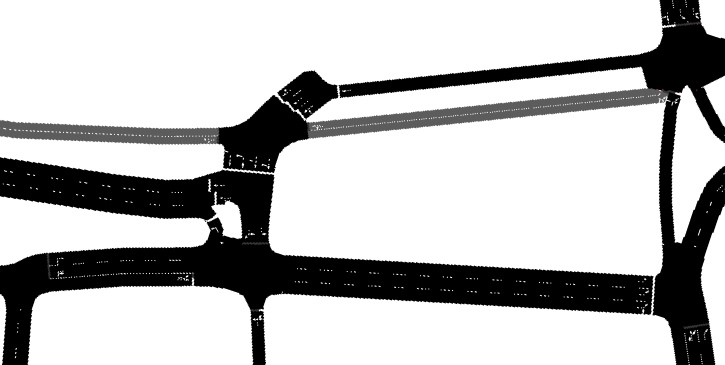
\includegraphics[width=0.70\textwidth]{images/cenario_estudo_sumo.png}

    \par\vspace{0.25cm}
    \begin{minipage}{0.70\textwidth}
        \footnotesize Fonte: Elaborado pelo autor.
    \end{minipage}
\end{figure}

\section{Construção e adequação da rede viária}

A rede inicial foi obtida a partir de dados do OpenStreetMap e convertida para o formato do \gls{sumo} com o \textit{netconvert}. A utilização de dados do OpenStreetMap como ponto de partida é compatível com o processo de construção de cenários descrito por \citeonline{clemente_2022}, que apresenta a preparação da rede, a definição do tráfego e o roteamento como etapas centrais de uma microssimulação no SUMO.

Após a conversão, a rede foi inspecionada e ajustada manualmente no \textit{NetEdit}. O objetivo dessa etapa foi obter uma representação funcional da circulação da região, e não preservar automaticamente todos os elementos importados. Foram removidos trechos externos sem função no experimento e corrigidos sentidos de circulação, conexões entre faixas, permissões de conversão, prioridades e geometrias que não estavam adequadas ao recorte utilizado.

Também foram revisadas as velocidades das vias. Na configuração utilizada nos experimentos, os limites ficaram concentrados em 40 km/h na região central e 50 km/h em trechos externos ou vias principais compatíveis com esse limite.

Um ajuste localizado foi realizado na região de acesso ao bairro Matriz, pela Rua Saul Brandalise. Na rede inicialmente importada, um veículo aguardando para realizar uma conversão à esquerda podia bloquear completamente o fluxo que seguia pela via. A observação do local mostrou a existência de um pequeno espaço utilizado para aguardar a conversão sem impedir necessariamente a passagem dos demais veículos. A geometria simulada foi então modificada para representar essa condição de forma simplificada.

A versão final da rede foi mantida em \texttt{config/nereu\_ramos.net.xml}. Versões anteriores foram preservadas no repositório do projeto para permitir rastrear os ajustes realizados durante o desenvolvimento.

\section{Verificação funcional do cenário}

Antes da definição dos experimentos, foram realizadas execuções preliminares para verificar se a rede permitia circulação contínua e se as conexões configuradas produziam trajetos válidos. Nessa etapa foram observados principalmente o funcionamento das entradas e saídas, o comportamento nos cruzamentos, as mudanças de faixa, as conversões e a formação de filas.

Os primeiros testes utilizaram viagens geradas com o \textit{randomTrips.py}. Essa estratégia foi útil para encontrar problemas de conectividade e comportamento da rede, mas também evidenciou uma limitação: uma distribuição totalmente aleatória atribuía tráfego excessivo a algumas vias secundárias e produzia uma utilização pouco plausível dos acessos da região. Por esse motivo, a geração de demanda foi posteriormente substituída por um procedimento controlado, descrito na seção seguinte.

A verificação também incluiu a observação de eventos que poderiam indicar problemas de configuração, como colisões, frenagens de emergência, bloqueios persistentes e \textit{teleports}. Os testes permitiram corrigir problemas localizados antes do congelamento da rede utilizada nos experimentos.

Durante a inspeção visual foi identificada ainda uma tendência de alguns veículos realizarem mudanças estratégicas de faixa com antecedência. Foram testadas alterações globais relacionadas ao comportamento estratégico de mudança de faixa, mas elas não produziram melhora suficiente para justificar sua adoção e, em alguns casos, introduziram instabilidade. Por esse motivo, a configuração-base foi mantida e essa característica foi considerada uma limitação conhecida da representação simulada.

\section{Definição e geração da demanda}

A demanda utilizada no experimento foi construída de forma controlada. O objetivo não foi reproduzir contagens reais de tráfego, pois não foi realizada uma coleta de fluxo veicular na região, mas evitar que a distribuição das viagens fosse completamente aleatória e pouco coerente com a importância relativa das vias do recorte.

As origens e os destinos foram definidos a partir dos acessos disponíveis na rede e receberam pesos relativos. As vias de maior importância no recorte receberam maior probabilidade de seleção, enquanto acessos secundários receberam pesos menores. Esses pesos representam apenas uma relação de importância entre os acessos e não correspondem a volumes reais medidos.

A Tabela~\ref{tab:pesos-demanda} apresenta os pesos utilizados na configuração final da demanda.

\begin{table}[H]
\centering
\caption{Pesos relativos utilizados na geração da demanda}
\label{tab:pesos-demanda}
\small
\renewcommand{\arraystretch}{1.20}
\begin{tabular}{|p{6.2cm}|c|c|}
\hline
\textbf{Via ou acesso} & \textbf{Peso como origem} & \textbf{Peso como destino} \\
\hline
Rua Saul Brandalise & 5 & 6 \\
\hline
Avenida Dom Pedro II & 5 & -- \\
\hline
Rua XV de Novembro -- acesso principal & 5 & 5 \\
\hline
Rua XV de Novembro -- acesso secundário & 3 & 4 \\
\hline
Rua Brasil & 3 & 3 \\
\hline
Rua Antônio Marafon & 2 & 1 \\
\hline
Rua Antônio Fávero & -- & 2 \\
\hline
Rua Osvaldo Cruz & 1 & 1 \\
\hline
Rua Santa Catarina & 1 & -- \\
\hline
Rua Padre Anchieta & -- & 1 \\
\hline
Rua Farroupilha & 1 & 1 \\
\hline
Rua Nicolau Cavon & 1 & 1 \\
\hline
Rua Sete de Setembro & -- & 1 \\
\hline
Rua Duque de Caxias & -- & 1 \\
\hline
\end{tabular}

\par\vspace{0.25cm}
\begin{minipage}{\textwidth}
\footnotesize Fonte: Elaborado pelo autor.
\end{minipage}
\end{table}

Além dos pesos individuais, alguns pares origem--destino receberam fatores de redução para diminuir a ocorrência de viagens que retornavam pelo mesmo corredor ou produziam deslocamentos pouco interessantes para o cenário. Em geral, retornos pelo mesmo corredor utilizaram fator 0,2. Os pares entre Rua Saul Brandalise e Rua Brasil, nos dois sentidos, utilizaram fator 0,6. Esses fatores reduzem a probabilidade de seleção dos pares, mas não os proíbem.

A geração foi implementada no script \texttt{scripts/gerar\_demanda\_v2.py}. Para cada execução, o script recebe a quantidade de veículos e uma semente pseudoaleatória. Os horários de partida são distribuídos uniformemente ao longo do intervalo de 0 a 600 segundos. Em seguida, a origem é sorteada de acordo com seus pesos e o destino é selecionado por uma distribuição ponderada condicionada à origem, considerando também os fatores aplicados aos pares penalizados.

Depois da geração das viagens, o \textit{duarouter} é utilizado para calcular rotas válidas na rede. O próprio processo verifica se a quantidade de rotas geradas corresponde à quantidade de veículos solicitada. Dessa forma, a aleatoriedade permanece na escolha das origens e destinos, mas ocorre dentro de uma estrutura de demanda controlada e reproduzível pela semente utilizada.

\section{Testes preliminares e ajustes de plausibilidade}

Durante os testes preliminares, um dos pontos que exigiu maior atenção foi o comportamento dos veículos em aproximações sem prioridade. Em determinadas situações, veículos permaneciam aguardando por períodos considerados excessivos mesmo quando existiam oportunidades visuais de entrada no fluxo prioritário. Esse comportamento produzia filas persistentes que dificultavam avaliar se a retenção era consequência da demanda ou da própria configuração do modelo de interseção.

Foram então avaliados parâmetros relacionados à aceitação de oportunidades em cruzamentos. O parâmetro global \texttt{time-to-impatience}, que controla a evolução da impaciência durante a espera, foi ajustado após testes comparativos. Na configuração final foi adotado o valor de 45 segundos. Também foi utilizado \texttt{jmTimegapMinor = 0.80}, relacionado ao intervalo temporal mínimo considerado na interação com veículos prioritários.

Esses valores não foram obtidos por calibração com dados reais da região. Eles foram mantidos como ajustes de plausibilidade após os testes mostrarem redução de esperas excessivamente conservadoras sem introduzir instabilidade generalizada na rede. A distinção é importante porque uma calibração empírica exigiria dados observados para comparar diretamente os comportamentos simulados com o trânsito real.

Outros parâmetros globais também foram mantidos constantes após essa etapa. O passo da simulação foi definido em 0,1 segundo, os \textit{teleports} foram desativados e a verificação de colisões em cruzamentos foi habilitada. Essas configurações permaneceram iguais entre os cenários para evitar que alterações no funcionamento básico do simulador interferissem na comparação entre os perfis de motoristas.

\section{Definição dos níveis de demanda}

A definição dos níveis de demanda foi realizada por meio de testes progressivos de carregamento da rede. O objetivo foi selecionar condições que representassem diferentes intensidades de circulação sem utilizar como cenário principal uma carga que produzisse congestionamento persistente ou impedisse a conclusão das viagens em determinadas realizações aleatórias.

Após os testes preliminares, foram definidos três níveis para o experimento: 300 veículos no nível baixo, 450 veículos no nível médio e 625 veículos no nível alto. Em todos os casos, os veículos são gerados durante a mesma janela de 600 segundos.

\begin{table}[H]
\centering
\caption{Níveis de demanda utilizados nos experimentos}
\label{tab:niveis-demanda}
\small
\renewcommand{\arraystretch}{1.20}
\begin{tabular}{|p{5cm}|c|c|}
\hline
\textbf{Nível} & \textbf{Veículos} & \textbf{Janela de geração} \\
\hline
Baixo & 300 & 0--600 s \\
\hline
Médio & 450 & 0--600 s \\
\hline
Alto & 625 & 0--600 s \\
\hline
\end{tabular}

\par\vspace{0.25cm}
\begin{minipage}{\textwidth}
\footnotesize Fonte: Elaborado pelo autor.
\end{minipage}
\end{table}

O nível de 300 veículos representa a condição de menor carregamento adotada no estudo. O nível de 450 veículos foi utilizado como condição intermediária. Para o nível alto, testes adicionais foram realizados com 625, 650, 675, 700 e 750 veículos. A carga de 625 veículos apresentou funcionamento estável nas repetições avaliadas durante o desenvolvimento, enquanto cargas superiores passaram a apresentar congestionamentos persistentes em algumas combinações de demanda e composição comportamental.

Por esse motivo, 625 veículos foi mantido como o nível alto do experimento principal. Essa escolha evita que o cenário de maior carregamento seja definido por uma condição em que parte das execuções deixa de representar apenas diferenças comportamentais e passa a ser dominada por um estado de congestionamento persistente da rede.

Com a rede, a demanda e os níveis de carregamento definidos, a configuração do cenário experimental foi congelada para a etapa seguinte. O próximo capítulo apresenta a parametrização dos perfis de motoristas, as composições utilizadas e o procedimento de execução das simulações.
